% !TEX root =  CurvedFoldedDogs.tex

\section{Folding crease patterns} \label{sec:folding}
In this section we explore the different ways one can fold a given crease pattern. Our result is a discrete combinatorial characterization for the local existence of a fold in a piecewise DOG.

%Two intersecting developable surfaces can be flattened along their intersection if the intersected curve have the same geodesic curvature on both surfaces. 
\subsection{The smooth and combinatorial degrees of freedom around a single curved crease}
\label{sec:smooth-combinatorial}

Straight creases are rather boring, mathematically speaking. Straight lines can only be folded as in classical origami, i.e., by keeping them straight \cite{demaine_lens}. \OSH{Or Tim's comment -- if the line becomes curved, it means that we have a ``double cover'', i.e., we folded 180 degrees and the two sheets coincide completely now.} Hence a folding of a single straight crease can be described by a single real number representing the constant dihedral angle between the incident planes. There are infinite many ways, or degrees of freedom, to fold a curved crease. If $S$ is a surface with a folded crease, and $P$ is its flattened isometric reference, then one can locally deform the curved surface by freely deforming the crease curve, as long as the absolute value of the crease curvature stays bigger than its flattened curvature at $P$ \cite{more_on_paper}. Up to rigid motion a curve is defined by its curvature and torsion functions.

One can flip this point of view: Given a planar domain $P$, a curve on the domain $\gamma(t)$ and a deformed space isometric curve $\Gamma(t)$ with a larger absolute curvature than $\gamma(t)$, there are only two smooth surfaces isometric to $P$ passing through $\Gamma(t)$ such that the unfolding of the surface to the plane maps $\Gamma(t)$ to $\gamma(t)$ \cite{mathematical_omnibus} (see \figref{fig:folding_combinatorics} left and center).


%To see that, assume that $S$ is such a surface; assume a crease pattern consisting of a single crease such that $S = P_1 \cup P_2$ (\figref{fig:folding_combinatorics} left). Let $\Gamma(t) = P_1 \cap P_2$ be the 3D crease curve and $\gamma(t)$ its flattening in $P$. Let $\kappa(t)$ be the curvature of $\Gamma(t)$ and $\kappa_g(t) = \kappa(t) \cos(\alpha(t))$ be its geodesic curvature \OSH{who is $\alpha(t)$?}. Assume that the curve is bent further in space, i.e., $\kappa(t) > \kappa_g(t)$. Then the tangent planes of $P_1$ and $P_2$ form an angle of $2\alpha(t) \neq 0$ with the osculating plane of $\Gamma(t)$ \cite{more_on_paper,duncan_folded}. Since $P_1,P_2$ are $C^2$,  there are four options for a consistent choice of a family of tangent planes along each side of the crease $\Gamma(t)$. Two of these four options correspond to a folding (i.e., tangent discontinuity) by choosing one family tangent planes along $\Gamma(t)$ for $P_1$ and the other for $P_2$ (see \figref{fig:folding_combinatorics}).
\begin{figure} [h]
	\centering
	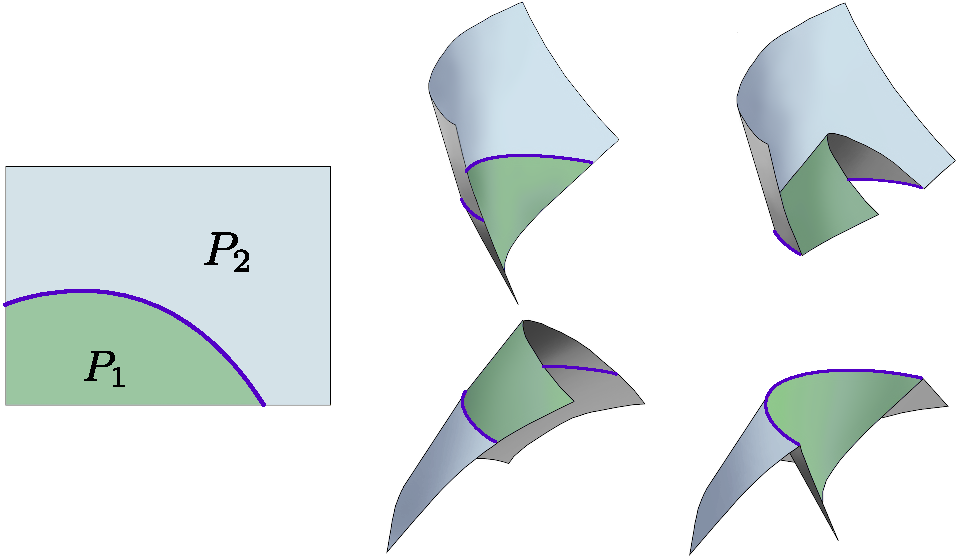
\includegraphics[width=\linewidth]{figures/curved_fold_through_curve_1.pdf}
	\caption{Illustration of the combinatorial degrees of freedom in curved folding. If a crease pattern of a curved folded surface (left) is isometrically folded such that a given curve lies in some configuration in $\R^3$, then there are only two smooth surfaces that isometrically flatten into the crease pattern (center). One can also choose a different surface for each patch $P_1,P_2$, resulting in two other, curved folded surfaces (right).}
	\label{fig:folding_combinatorics}
\end{figure}

If one permits the surface $S$ to have a fold along $\Gamma(t)$ but still stay smooth around it, then there are four possible surfaces: two of them are smooth, while two of them are folded along the curve (see \figref{fig:folding_combinatorics}). If $S = S_1 \cup S_2$ is folded along $\Gamma(t) = S_1 \cap S_2$ then the angle between the tangent planes of $S_1,S_2$ along the curve is called the folding angle, which we denote by $\theta(t) > 0$. Unlike the case of a straight crease, $\theta(t)$ often varies along the curve.  The bigger the curvature of $\Gamma(t)$, the bigger the folding angle. If $\kappa(t)$ is the curvature of the space curve $\Gamma(t)$, $\kappa_g(t)$ is its geodesic curvature, which is also the curvature of $\gamma(t)$, then $\kappa(t) = \cos\frac{\theta}{2},$ implying that the osculating plane of the crease $\Gamma(t)$ bisects the tangent planes of the smooth patches intersecting at $\Gamma(t)$ \cite{curved_folding_kilian,duncan_folded}. The folding angle does not dictate the shape of the surface, as different surfaces can be generated with the same $\theta(t)$ by varying the torsion of $\Gamma(t)$, thereby changing the ruling pattern of each developable patch. The connection between $\theta(t)$, the curvature and the torsion of $\Gamma(t)$, the curvature of $\gamma(t)$ and the rulings of each incident patch is further detailed at \cite{demaine2018conic}.

To summarize, the shape of a curved folded surface $S$ with a single curved crease $\Gamma(t)$ can be locally described by two {real functions} for the curvature and torsion of $\Gamma(t)$ under the condition of sufficient absolute curvature, as well as an additional combinatorial parameter distinguishing between four possible surfaces, two of which have a fold.
 
\subsection{The combinatorial parameters of multiple creases}
The previous analysis explains the local behavior of curved folding around a single curve. Understanding crease patterns globally still remains a challenge. In essence, deforming one patch propagates a global deformation of the patch on the other side of the crease, a process that depends on the locations of the creases and the possibly changing ruling lines along the developable. When there are multiple creases, the propagation dictates the shape of other patches. The process becomes more complicated when some creases intersect, due to compatibility constraints (see \figref{fig:multiple_crease_patterns}). 

\begin{figure} [h]
	\centering
	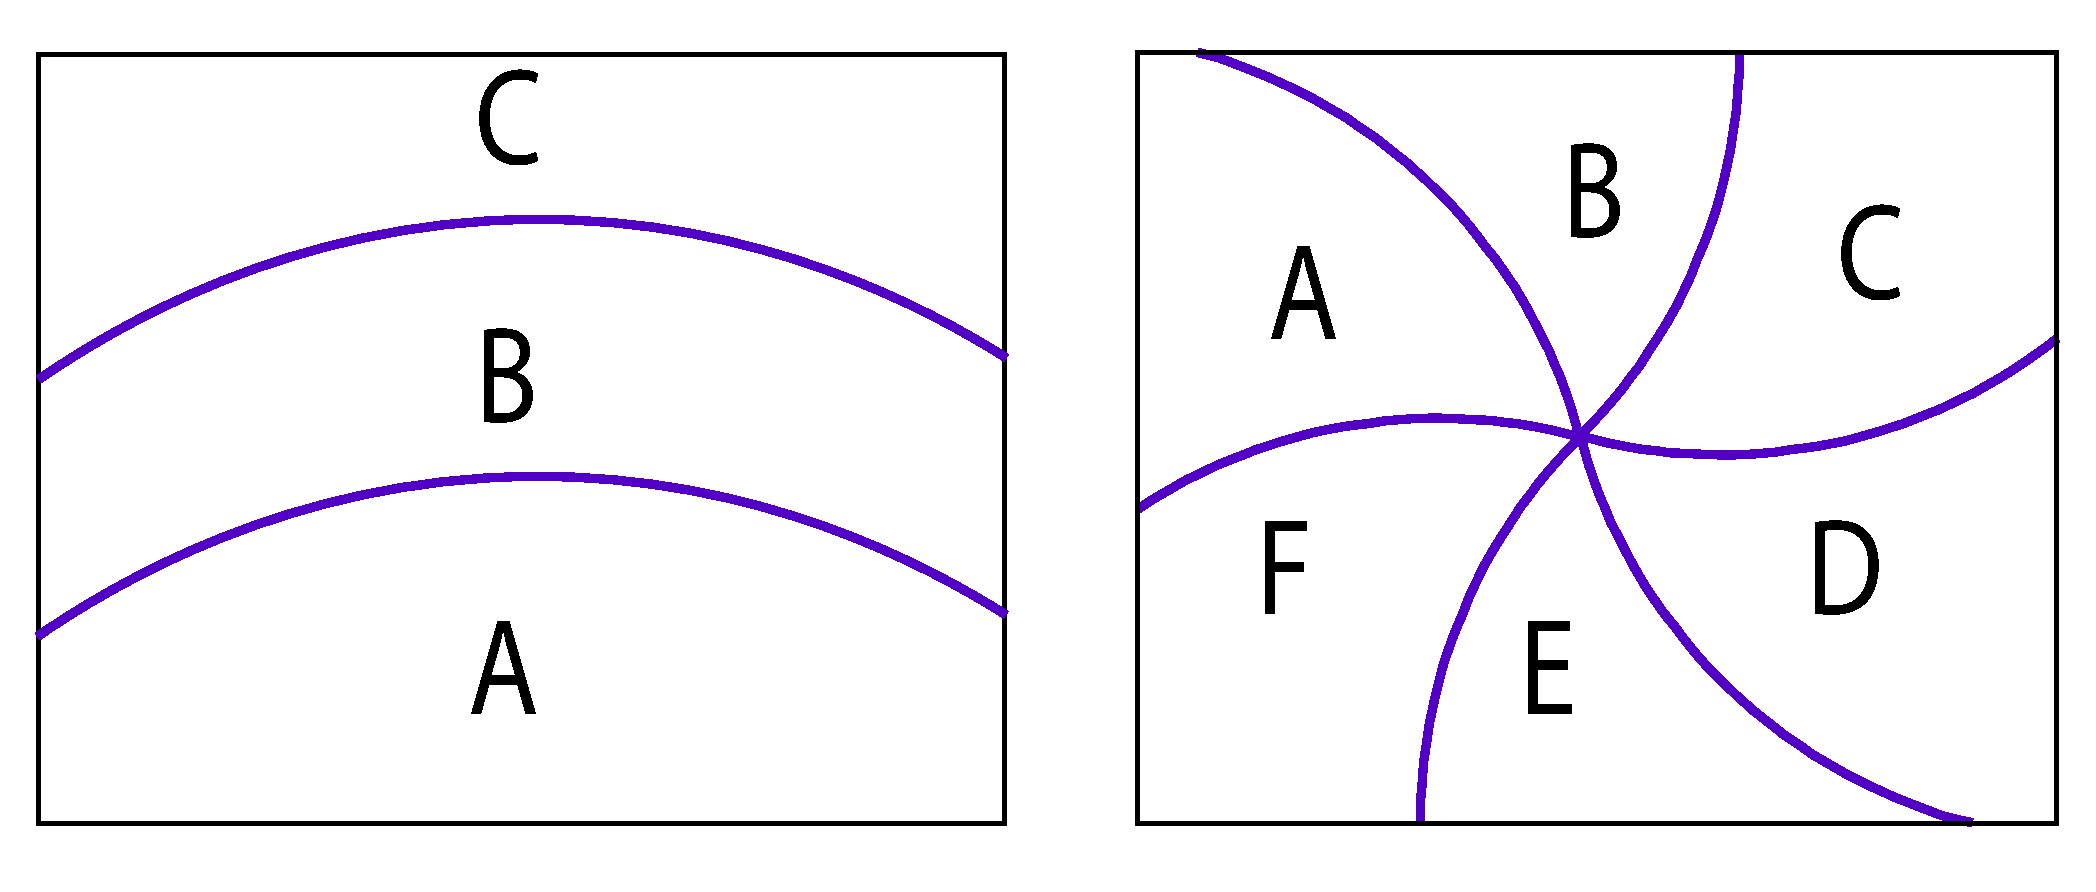
\includegraphics[width=\linewidth]{figures/multiple_crease_patterns}
	\caption{Propagation of constraints in crease patterns. Down: Crease patterns. Up: Curved folding of the crease patterns. Left and Center: A deformation in the patch $P_1$ dictates most of the shape of the patch $P_2$ which in turn dictates most of the patch of $P_3$. The propagation of deformation is generally global, and depends on the directions of the rulings. In these cases one can choose a mountain/valley assignment for one fold, which already determines the M/V assignment of the next fold (left: valley-mountain, center: valley-valley). Right: In more complicated crease patterns, for instance those with a vertex, the process is more complicated as there are also some compatibility conditions the patches need to satisfy. }
	\label{fig:multiple_crease_patterns}
\end{figure}

Generally speaking, one may be able to choose between four different configurations of the surface at one crease, but this choice already fixes the patch shape for nearby creases. The combinatorial degrees of freedom that remain are whether each crease is folded or not (see \figref{fig:folded_and_not_folded}). The difficulty in modeling folding of a planar surface stems from the fact that these combinatorial choices often need to be enforced at the beginning of the folding process, as explained by the following theorem.% combinatorial degree of freedom is often only available at the start of a deformation of a flat surface, as detailed in the following lemma:

\begin{theorem}\label{Thm:curved_folding_open_condition}
Let $S(t)$ be a curved folding flow and let $p(t_k)$ be a point on a curved crease of $S(t)$ lying on two patches $S_1(t),S_2(t)$ at a given time in the flow, $t=t_k$. If $p(t_k)$ is not a planar point on $S_1(t_k)$ (or equivalently on $S_2(t_k)$), then there exists an $\epsilon > 0$ such that one of the following holds:
\begin{enumerate}
	\item $\ S(t)$ is folded at $p(t)$ for every $t \in (t_k-\epsilon, \ t_k+\epsilon)$;
	\item $\ S(t)$ is \emph{not} folded at $p(t)$ for every $t \in (t_k-\epsilon, \ t_k+\epsilon)$.
\end{enumerate}
\end{theorem}
\begin{proof}
Let $\kappa(p(t))$ be the crease curvature at the point $p(t)$, and let $\kappa_g(p(t)) = \kappa(p(t))\cos\frac{\theta(p(t))}{2}$ be the crease's flattened (geodesic) curvature. If the folding angle $\theta(p(t)) \neq 0$, the claim follows from the discontinuity of the two tangent planes at $p(t)$: a folding corresponds to a different choice of the tangent planes, forming an angle of $\theta(p(t))$ with each other, and any small continuous deformation cannot move from a folded to a non-folded configuration or vice-versa. Finally, the non-planarity of $p(t_k)$ implies $\theta(p(t_k)) \neq 0$, since $\theta(p(t_k)) = 0$ would mean that the normal curvature of the crease curve is $0$, and therefore the tangent of the crease curve is parallel to the ruling direction.
% (see inset). 
But by Lemma 12 and Corollary 16 in \cite{demaine_lens} this implies that the curve has a kink at  $p(t_k)$, contradicting the fact that $S(t)$ is $C^2$ when restricted to the patches $S_1(t), S_2(t)$.
\end{proof}
%\setlength{\columnsep}{8pt}%
%\begin{wrapfigure}{r}{0.3\linewidth}
%  \centering
%  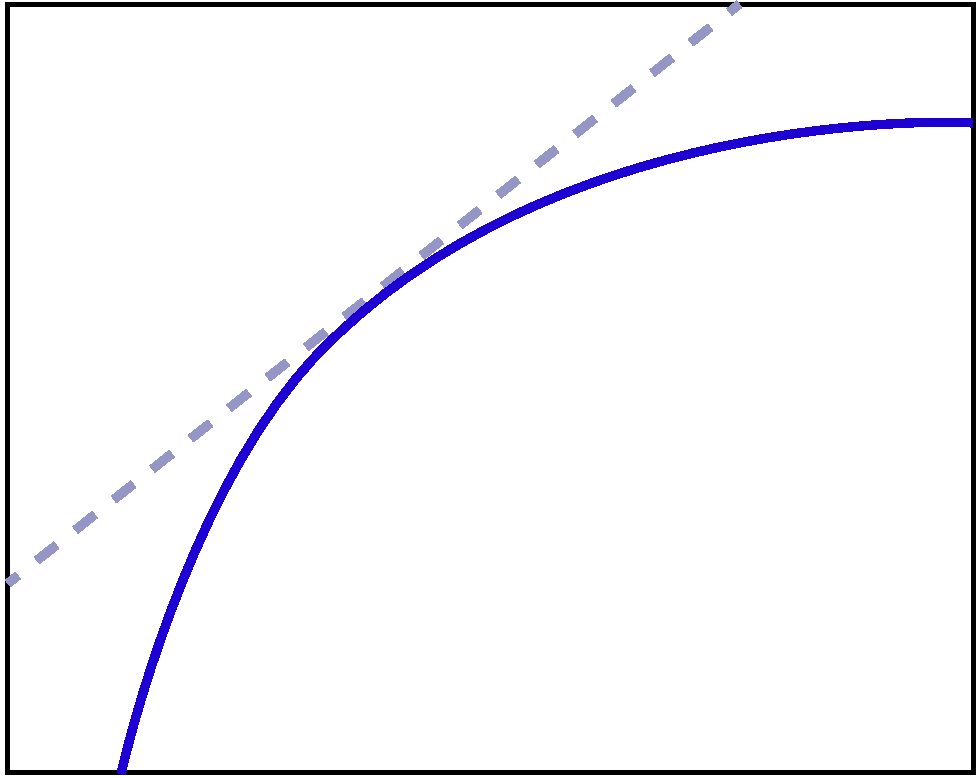
\includegraphics[width=\linewidth]{figures/ruling_tangent_to_a_curved_fold}
%%  \caption{\label{fig:cone_from_curve} A local representation of a developable surface through a curvature line curve $\gamma(s)$, and orthogonal rulings emanating from it.}
%\end{wrapfigure}

Therefore it is impossible to fold a crease point that is non-planar. For a non-planar point that is not folded, any small deformation keeps it that way. Folding can only happen after flattening the point, and if the surface is already folded, any small deformation keeps it folded. Thus, the decision whether to fold or not can only be done when the crease points are planar, while no extra care needs be taken if the crease is already folded. With this in mind, we note the following observation.

\begin{theorem}\label{Thm:supporting_plane}
A non-planar curved crease point $p$ on a curved folded surface $S$ is folded if and only if the osculating plane of the crease curve at $p$ is locally a supporting plane for the patches $S_1,S_2$ intersecting at $p$.
\end{theorem}
\setlength{\columnsep}{8pt}%
\begin{wrapfigure}{r}{0.2\linewidth}
  \centering
  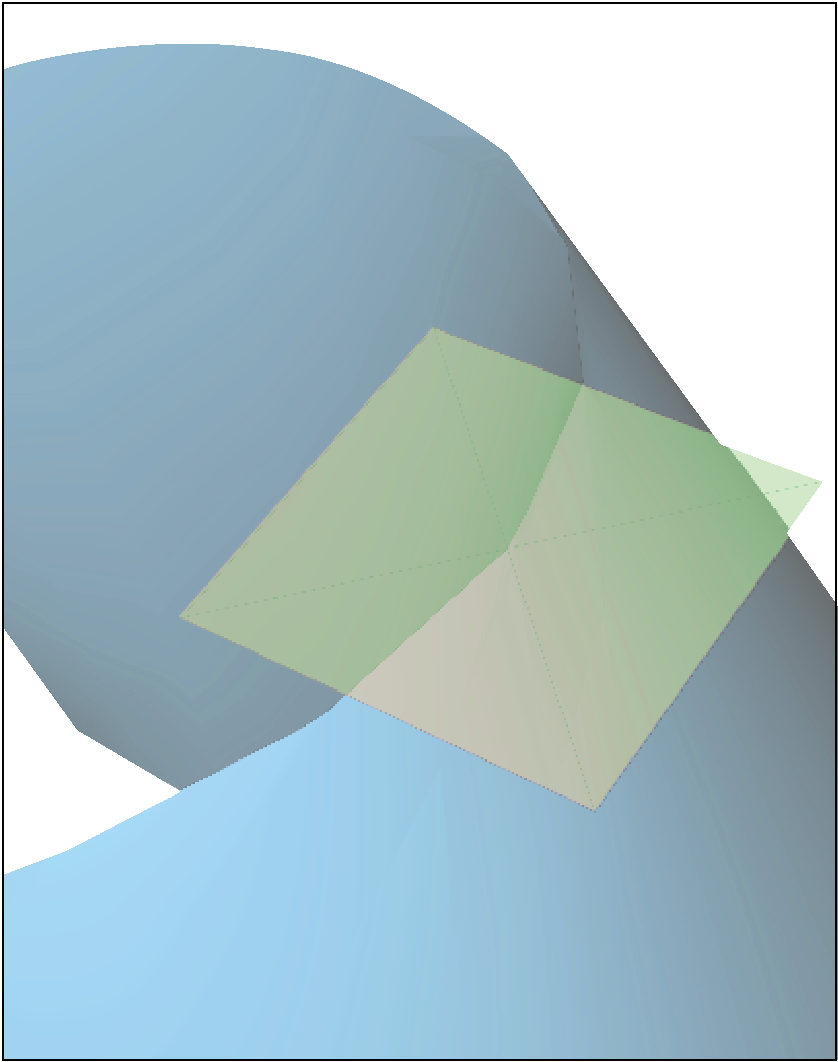
\includegraphics[width=\linewidth]{figures/plane_side.pdf}
\end{wrapfigure}
This follows directly from the fact that the tangent planes on both sides of a crease curve coincide if the surface is smooth there, but along a folded crease they are reflections of one another through the crease curve's osculating plane. Planar crease points along a curved crease, while not folded, still satisfy this constraint, since around these points the tangent planes are exactly the same as the osculating plane of the curve, though even the slightest surface deformation might change that. 

\subsection{Discretization}
We saw that folding happens exactly when both sides of the surface around a crease are in the same half-space of the osculating plane of the crease curve. We discretize this condition by constraining the tangents of the discrete parametric (grid) lines of the two DOG patches to be on the same side of the crease curve's discrete osculating plane. See \figref{fig:osc_plane_discretization} for the notation. The DOG edges intersecting the crease can be considered as discrete surface tangents originating at the crease points. In the notation of \figref{fig:osc_plane_discretization}, each of the two patches has its own duplicate of the edge ($e_1$ or $e_2$) intersecting the crease curve. In the starting, flat configuration the two edges coincide, but a folding movement creates a discontinuity between them. We denote the discrete surface tangents on both sides of the crease curve as $t_1 = \frac{e_1}{\|e_1\|}, t_2 = \frac{e_2}{\|e_2\|}$. The binormal of the crease curve, i.e., the normal of its osculating plane, is $B = \frac{e_f \times e_b}{\|e_f \times e_b\|}$, noting that $e_f,e_b$ always coincide for both patches.

\begin{figure} [h]
	\centering
	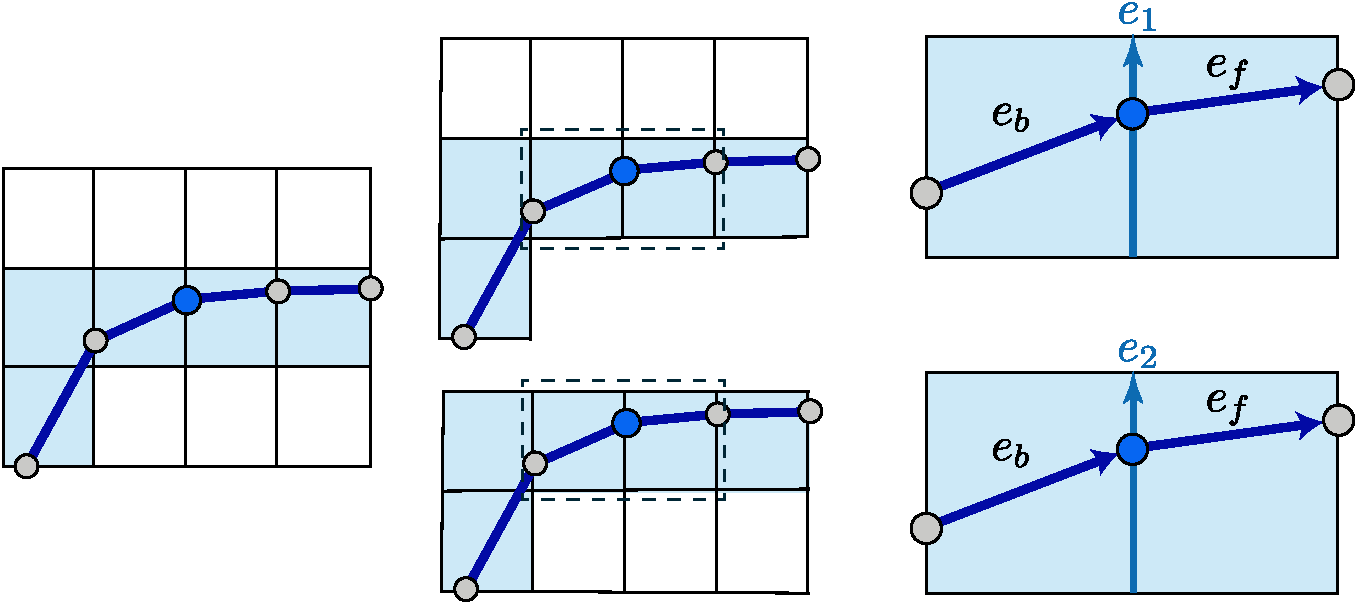
\includegraphics[width=\linewidth]{figures/osc_plane_discretization}
	\caption{Notation for edges in a discrete crease pattern. Left: a DOG net with a discrete crease curve. Center: Following \cite{rabi2018shape}, we represent creases by duplicating the quads that contain the crease curve, which results in different connected components, or patches. The positions of the vertices on the curve, i.e., its intersection points with the grid edges, are constrained to match on both patches. Right: Notation for a duplicated grid edge ($e_1, e_2$) intersecting the crease curve at the blue point(s), and the two crease edges $e_f,e_b$. }
	\label{fig:osc_plane_discretization}
\end{figure}

The supporting plane constraint can be written as
\begin{equation} \label{eq:folding_const_normalized} 
\text{sgn}(\langle t_1,B\rangle) +  {sgn}(\langle t_2,B\rangle) = 0
\end{equation}
with 
\begin{equation} \label{eq:sign}
\text{sgn}(x) = \left\{
     \begin{array}{@{}r@{\thinspace}l}
       -1  &: \text{if } x < 0, \\
       0 &: \text{if } x = 0, \\
       1 &: \text{if } x > 0. \\
     \end{array}
   \right.
\end{equation}
%
Constraint \eqref{eq:folding_const_normalized} can be simplified by replacing $B$ with the cross product $e_f \times e_b$. Furthermore, if one assumes an isometric deformation, it is possible to replace $t_1,t_2$ by the non-normalized edges $e_1,e_2$, arriving at:
\begin{equation} \label{eq:folding_const}
\text{sgn}(\langle e_1,e_f \times e_b \rangle) +  {sgn}(\langle e_2,e_f \times e_b\rangle) = 0.
\end{equation}
In \secref{sec:implementation} we show how to plug this constraint into an optimization framework to model folding and bending of curved folded DOGs (see \figref{fig:folded_and_not_folded}).

\subsection{Discussion}
There are multiple equivalent characterizations for a folded crease over a curved folded surface. We now point out some key properties of our chosen discretization \eqref{eq:folding_const_normalized} and briefly discuss how these properties elude other possible constraint choices.

\paragraph{Suitable for homotopy based optimization methods} 
Our constraint is satisfied on a flat mesh. In this sense we consider a point along a curve with zero normal curvature as both folded and not folded.
 
\paragraph{Minimal and generally non-intrusive} 
Once a curved crease on a piecewise DOG is folded, one no longer needs to take explicit care for it to stay folded. The effect of \equref{eq:folding_const} on an already folded surface is null. The tangent discontinuity caused by the folding implies that a folded crease remains folded under local deformations, and in order for it to become unfolded, one need to first flatten it, as is the case for a piecewise smooth curved folded surface. We also capture the converse: a discrete curved crease can only be folded when starting from a planar point (\theoremref{Thm:curved_folding_open_condition}). \\

An alternative constraint for folding could be e.g.\ enforcing discontinuities along the tangents $t_1,t_2$, but this results in losing the feasibility of the flat models. Moreover, in the discrete case a minor discontinuity can still arise even though there is no fold, i.e., where \equref{eq:folding_const_normalized} is not satisfied, thus numerically giving the impression of a fold when visually there is none. Another option is to define folded configurations as those satisfying a similar but simpler smooth constraint:
%
\begin{equation} \label{eq:folding_const_smooth} 
\langle t_1,B\rangle + \langle t_2,B\rangle = 0.
\end{equation}
%
This condition is satisfied exactly in flat models and in any piecewise smooth curved folded surface, since tangent planes along a folded creased curve are reflections of each other w.r.t.\ the osculating plane of the crease curve. However, this condition is not satisfied \emph{exactly} on every folded piecewise DOG (as evident by all models in this paper). An exception to this is the class of curved creases with zero torsion, in which case the folds are simply formed as a global plane reflection \cite{Mitani_ref}. Therefore, enforcing constraint \eqref{eq:folding_const_smooth} as a hard constraint is too restrictive in practice, while enforcing it softly creates a condition that, unlike the smooth case, does not vanish once a crease is folded and hence is not minimal in our sense.


\section{Folding angles and mountain-valley assignments} \label{sec:folding_angles_mountain_valley}

In this section we propose tools to constrain the folding angles and their direction (mountain or valley) during deformation, in order to provide designers with additional expressive and intuitive control. We first show how to constrain folding angles, i.e., the angles between the tangent planes around a crease. We implement this by constraining DOG tangent angles, resulting in a simple quadratic constraint. We then devise a tool to differentiate between mountain and valley folds. Our derivations work for both curved and straight origami creases.

\subsection{Folding angle} 

A folding deformation can be seen as a rotation of the surface patches' tangent planes hinged on the tangent of the crease curve. The tangent of a straight fold is constant, and so is the folding angle, while on a curved crease, the tangent varies and often the folding angles change along the crease. In both cases, if the folding angle at a given point is $\theta$, then the surface tangent vectors on both sides of the crease that are orthogonal to the crease tangent form an angle of $\theta$, while the surface tangent vectors that are parallel to the crease remain parallel to each other. The following lemma shows the relation between the angle formed by surface tangent vectors that are equal in the flattened configuration and the folding angle (see \figref{fig:fold_angle_and_tangent_angles}): 
 \begin{lemma}  \label{lem:tangents_dihedral}
 Let $t_1,t_2$ be surface tangent vectors on two sides of a crease curve at a given point $p$ that are equal to each other in the isometrically flattened state of the developable surface. Let $t$ be the crease curve tangent at $p$. Assuming the surface went through a curved folding isometric deformation and the folding angle at crease point $p$  is $\theta$, the surface tangent vectors satisfy:
\begin{equation} \label{eq:tangents_dihedral}
\langle t_1, t_2 \rangle = \cos^2\!\alpha + \sin^2\!\alpha \cos\theta, \end{equation}
%4*cos(alpha/2)/(norm(e1)+norm(e2))
where $\alpha$ is the angle between $t$ and $t_1$. Note that this angle is preserved under isometry.
\end{lemma}
\begin{proof}{We denote by $t,n,b$ the vectors of the Frenet frame of the curved crease at $p$. We wish to express the surface tangent vectors $t_1, t_2$ in the local coordinates of this Frenet frame. In the flat isometric configuration, $t_1, t_2$ coincide and can be written as $\cos(\alpha)t + \sin(\alpha)n$. A folding angle of $\theta$ means that relative to the Frenet frame of the curve, the surface tangent on one side of the curve was rotated by angle $\frac{\theta}{2}$ about the crease curve tangent $t$, and the surface tangent on the other side by  $-\frac{\theta}{2}$. 
%
Thus w.l.o.g.\ 
\begin{align*}
\textstyle t_1 = \cos(\alpha)t + \sin(\alpha)\left(\cos\left(\frac{\theta}{2}\right)n + \sin\left(\frac{\theta}{2}\right)b\right),\\
\textstyle t_2 = \cos(\alpha)t + \sin(\alpha)\left(\cos\left(\frac{\theta}{2}\right)n - \sin\left(\frac{\theta}{2}\right)b\right). 
\end{align*}
%
The proof is concluded by computing $\langle t_1,t_2 \rangle$ and plugging in the trigonometric identity $\cos\theta = \cos^2{\frac{\theta}{2}}-\sin^2\frac{\theta}{2}$.}\end{proof}

Under an isometric deformation, $t_1,t_2$ are linear in the vertex positions, $\alpha$ is constant and  \equref{eq:tangents_dihedral} is quadratic.

\begin{figure} [h]
	\centering
	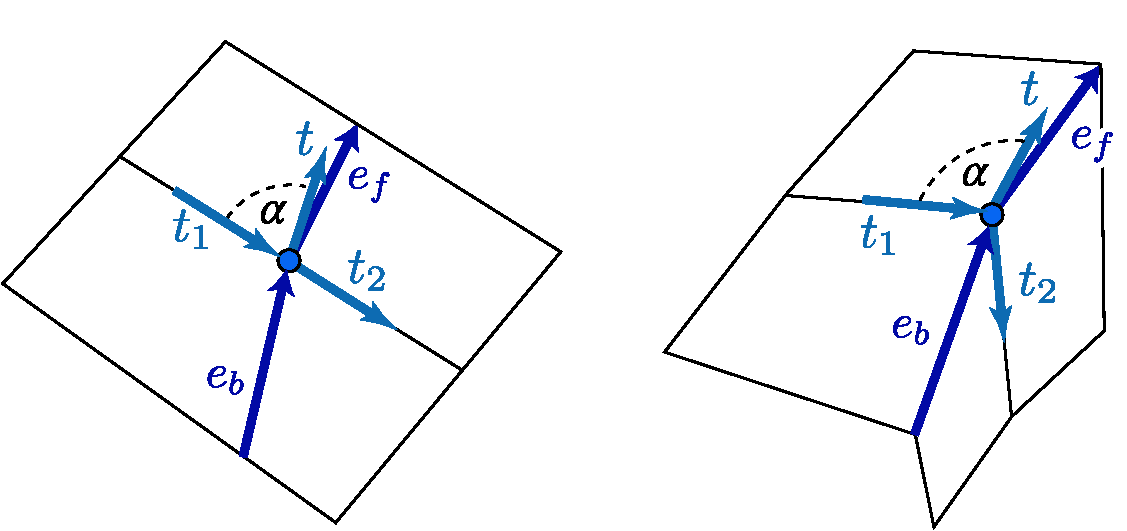
\includegraphics[width=0.8\linewidth]{figures/fold_angle_and_tangent_angles}
	\caption{Left: A flattened configuration of a crease curve (dark blue) with edges $e_f,e_b$ and its tangent $t$, forming an angle $\alpha$ with the DOG tangents $t_1,t_2$, which are equal in this flat state ($t_1=t_2$). Right: A folded isometric configuration with a tangent discontinuity  $t_1 \neq t_2$. \lemmaref{lem:tangents_dihedral} shows the connection between the angle $\alpha$ and the folding angle $\theta$ in the smooth case, stating that $\langle t_1, t_2 \rangle = \cos^2\!\alpha + \sin^2\!\alpha \cos\theta$. \OSH{For illustrating the lemma, it's better to put a smooth picture.}}
	\label{fig:fold_angle_and_tangent_angles}
\end{figure}

\subsection{Mountain/valley assignments} 
As mentioned in \secref{sec:smooth-combinatorial}, there are a few combinatorial degrees of freedom in choosing the type of fold, i.e., the choice of surfaces on each side of the curve (\figref{fig:folding_combinatorics}). We follow \cite{demaine_lens} to distinguish between the two types of folded configurations in \figref{fig:folding_combinatorics} by calling one choice a \emph{mountain fold} and the other a \emph{valley fold}. We would like to emphasize that for straight folds, this degree of freedom always exists, but on curved creases it often does not. In fact, in many crease patterns it is often only possible to choose one mountain/valley (M/V) assignment, and the remaining assignments are determined by the propagation of the rulings, leaving only the combinatorial degrees of freedom of whether a crease is folded or not, embodied by \equref{eq:folding_const_normalized}. 
%For instance, in \cite{demaine_lens} the authors prove how segments on the convex side of a crease bend mountain/valley the same as the crease, while segments on the concave side of a crease bend mountain/valley opposite from the crease. This can be seen in \figref{fig:multiple_crease_patterns}, where the left crease pattern has a mountain and valley fold while the center one has only valleys.
 We distinguish M/V folds by looking at whether a tangent of one surface patch is above or below the tangent plane of the second surface patch at the crease point, for a consistent choice of orientation. This can be achieved by the following constraint:
\begin{equation} \label{eq:mountain_valley_ineq}
\langle t_1, t \times t_2 \rangle \leq 0,
\end{equation}
where $t$ is the tangent of the oriented crease curve and $t \times t_2$ is the \OSH{normal of the?} tangent plane of the second surface patch (the one that has $t_2$ as a tangent vector). The orientation of $t$ determines whether a mountain or a valley fold is chosen. By the cyclic property of the triple product, the left hand side of \equref{eq:mountain_valley} \OSH{you meant \equref{eq:mountain_valley_ineq}, right?} is also equal to $\langle t_2, t_1 \times t \rangle$.
Using the notation of figure \figref{fig:fold_angle_and_tangent_angles}, we discretize the tangent of the crease curve at a given vertex by looking at the incident edge vectors $e_f, e_b$: 
$$t = \frac{\|e_b\|e_f + \|e_f\|e_b}{\left\|\|e_b\|e_f + \|e_f\|e_b\right\|}.$$
%
 If the two edge vectors $e_b, e_f$ are not collinear, $t$ as above is the tangent to the unique circle passing through the vertex and its two neighbors, taken at the vertex. It is a linear function of the vertices under isometry.
 
To simplify notation for \secref{sec:implementation}, we reformulate \equref{eq:mountain_valley_ineq} with equalities by using the Heaviside step function:
\begin{equation} \label{eq:heaviside}
\text{H}(x) = \left\{
     \begin{array}{@{}l@{\thinspace}l}
       0  &: \text{if } x \leq 0, \\
       1 &: \text{if } x > 0, \\
     \end{array}
   \right.
\end{equation}
and write the mountain/valley condition as:
\begin{equation} \label{eq:mountain_valley}
H(\langle t_1, t \times t_2 \rangle) = 0.
\end{equation}